\chapter{Preliminaries}
\label{ch:Preliminaries}

In this chapter we provide to the reader an introduction to the basic concepts of the theory we are using in order to develop our news-propagation model. Most of the topics in this chapter are provided more analytically in ~\cite{Kleinberg,IntroProbability,koller2009probabilistic,nisan_roughgarden_tardos_vazirani_2007} but we include the necessary background to make this thesis complete and provide the reader with a basic knowledge of the tools we used. We once again suggest the reader to further study the chapters from the above bibliography for more details.


\section{Branching Processes}
\label{sec:BranchingProc}

Epidemics is the most common structure based mitigation technique that is widely used in order to combat fake news propagation. Those models not only describe spread of viruses, but we can use them to formulate computer malware in networks and also information propagation such as the virality of social media posts. In this thesis, our building block is a refined version of branching process. Branching process is a simplistic version of epidemic and it works as follows:

\begin{itemize}
	\item \textbf{First wave} A person that is carrying a disease enters a population with $n$ individuals. With probability $p$ he transmits the disease to $k$ independently, i.e he meets three people and he infects only the first one.
	\item \textbf{Subsequent waves} Now, each infected person transmits the disease to their contacts, so the amount of susceptible people we have in the second wave is $k^2$ and in the $n$-th wave it is $k^n$ by induction. 
\end{itemize}	

\begin{figure}[t]
	\centering
	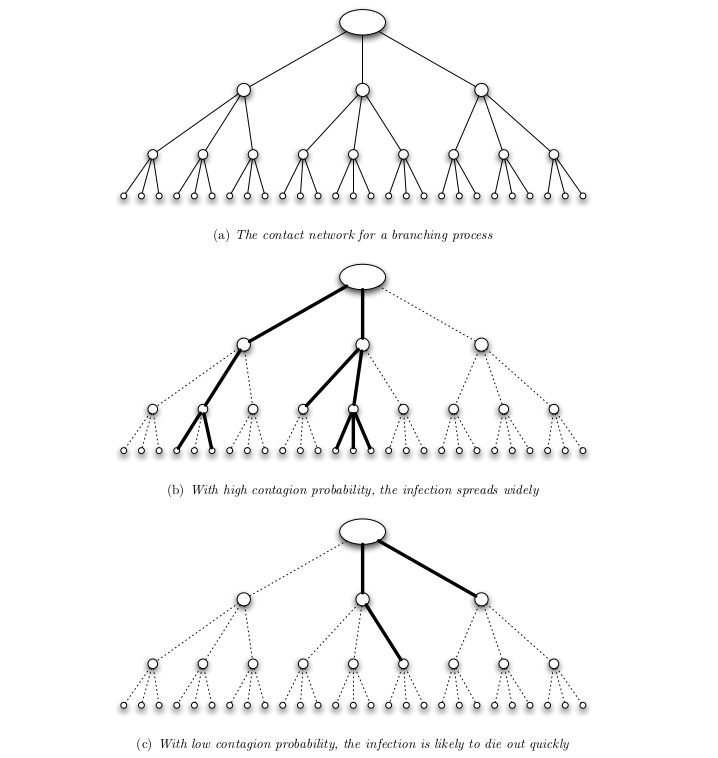
\includegraphics[width=.90\textwidth]{Figures/Selection_004.png}
	%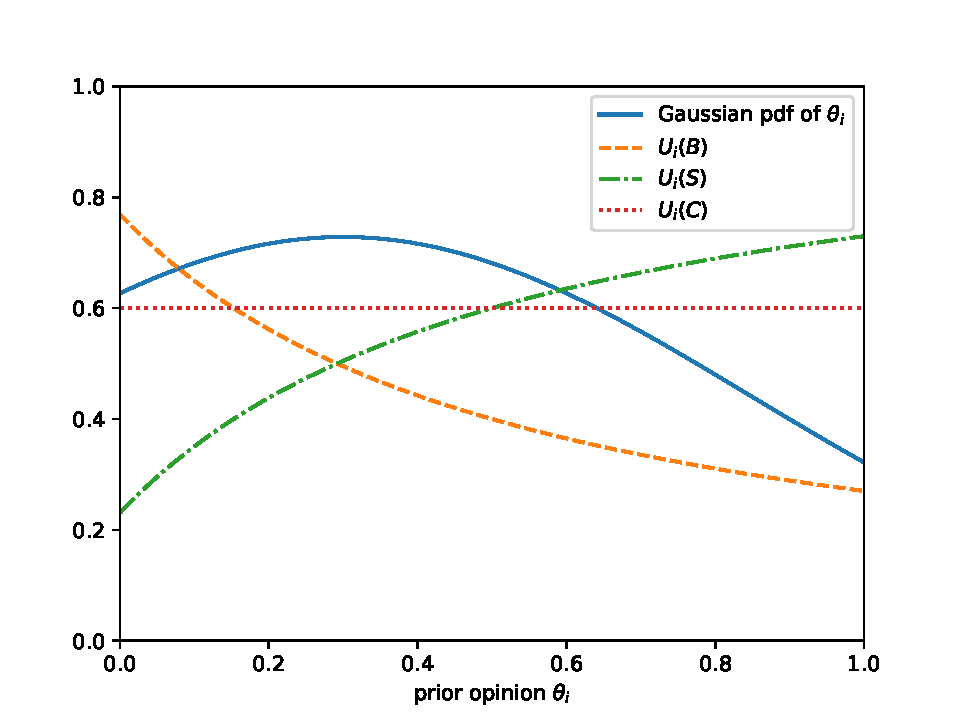
\includegraphics[width=.75\textwidth, height=.3\textheight]{Figures/line_plot.pdf}
	
	\caption{Branching process example with $k=3$. Reference in ~\cite{Kleinberg}.}
	
	\label{fig:branchProc}
\end{figure}

The above rules define a simple epidemic model where the probability of infections represents the rate and $k$ is the an average amount of a person's contacts. The question on those models is if the disease will survive (i.e., turn into a pandemic) or eventually stop spreading and die. The basic reproductive number determines whether a virus will continue spreading or if it fails. We have the next proposition from ~\cite{Kleinberg}:

\begin{prop}
	Let $R_0 = p k $ be the basic reproductive number where $k$ is the average people an individuals meets and $p$ is the probability that the virus spreads. If $R_0 \geq 1$, then with probability greater than zero the virus persists. If the basic reproductive number is less than $1$ then with probability $1$ the virus with stop spreading after some waves.
\end{prop}

The proof is provided more analytically in the related reference and it is based on geometric sequences, which will concern the more complex branching process later on the main body of this thesis. The reproductive number in our study can be translated as a prediction where we can tell if the process will trigger a cascade, given the contagion probability and the average people that a person \textit{meets}.

In our thesis we use a more complex version of that model. First of all, we do not have a fixed probability for infection. Every time nodes are added in the propagation tree, this probability is affected. Another modification we make on that model is the time that the process takes place. Instead of waves, we assume that each node contacts his neighbors at some time $t$, more later at the appropriate chapter. Although branching process seems significantly simpler than epidemics, it captures more with the correct modifications and that is the fact that it micro manage the contagion inside a network. In a nutshell, epidemics translate only the ratio at where entities move from a state to another and it does not account a change of probabilities.

\section{Bayesian Inference}
\label{sec:BayesianInf}

Bayesian inference is a statistical inference that update beliefs about uncertain parameters as more information becomes available. The Bayesian inference is one of the most successful methods used in decision theory, builds over Bayes’ theorem:
$$\mathbb{P}(H|E) = \frac{\mathbb{P}(E|H)\mathbb{P}(H)}{\mathbb{P}(E)}$$
which expresses the conditional probability of the hypothesis $H$ conditional to the event $E$ with the probability that the event, or evidence, $E$ occurs given the hypothesis $H$. In the previous expression, the posterior probability $\mathbb{P}(H|E)$ is inferred as an outcome of the prior probability $\mathbb{P}(H)$ on the hypothesis, the model evidence $\mathbb{P}(E)$ and the likelihood $\mathbb{P}(E|H)$ of the evidence $E$ occurring, given the validity of the hypothesis $H$. Bayes’ theorem has been widely used as an inductive learning model to transform prior and sample information into posterior information and is widely used in decision theory. In order to visualize the concept of Bayes theorem, we provide a simple example. Suppose people are tested for some disease. If the test is $99\%$ accurate, then this means that  $\mathbb{P}(Positive-test|Positive)  =  0.99$. However, the  most relevant information is $\mathbb{P}(Positive|Positive-test)$, namely the probability of having the disease if the test is positive, using Bayes theorem. If the proportion $\mathbb{P}(Positive)$ of infected people in the total population is $0.001$, then if we have the value of normalizing factor, i.e. $\mathbb{P}(Positive-test)=0.01$, and we conclude that $\mathbb{P}(Positive|Positive-test) = 0.099$, which provides different information and more relevant, using evidence rather than a simply using the accuracy of the test. It is obvious that both prior observations and the observable data, contain information, and so neither should be neglected. Bayes theorem has a general form as well, that works with multiple variables. The formula for discrete multiple variables, which we use in our thesis, is:

$$\mathbb{P}(H_k|E) = \frac{\mathbb{P}(E|H_k)\mathbb{P}(H_k)}{\sum_{i \in I} \mathbb{P}(E|H_i) \mathbb{P}(H_i)}$$
where ${H}_{i \in I}$ is partition of the sample space and $H_k$ is an observation inside that partition.

The process of drawing conclusions from available information is called inference.  However, in  many  cases the available information is often insufficient to  reach  certainty through reasoning.  In these cases, one may use different approaches for doing inductive inference. The strength of Bayesian inference, which is the method of using Bayes theorem to deduce a claim, is that it requires minimum but relevant information in order to work. This ability makes Bayesian inference an appropriate method to express how opinions are formed inside a social structure. Other notable applications are in medicine, machine learning, data analysis and many more.